\chapter{Experiments}\label{chapter:experiments}

In this chapter, we experiment with the training method we introduce in
Chapter~\ref{chapter:training_method}. This chapter's main goal is to show that our method improves the base student's performance and, ideally, also the performances of both teacher models. We also examine
each teacher's contribution to the student's performance and find a mix of the teachers' capabilities that produce the best-performing student model.

This chapter is laid out as follows. We describe the training data in
Section~\ref{section:val_training_data}. Next, we discuss how we compare models
in Section~\ref{section:validation_tasks}. In Section~\ref{section:student_model_config_baselines}, we present the student's
configuration and specify the baselines we try to beat in the following experiments. First, we experiment with the structural loss in Section~\ref{section:structural_loss}. Then, for the given best-performing structural loss, we find the best-performing contextual loss and
the weighting of the two losses in Section~\ref{section:structural_and_contextual}.
Finally, we summarize our experiments and findings in
Section~\ref{section:experiments_summary}.

\section{Training data}\label{section:val_training_data}

Our training dataset mirrors Longformer's training dataset, except for a few
exceptions. We have to leave out the Book corpus \citep{zhu2015aligning} and the Stories
corpus \citep{trinh2018simple} as they are currently unavailable. Thus, we
equally sample documents from English Wikipedia\footnote{\url{https://huggingface.co/datasets/wikipedia/viewer/20220301.en}} and RealNews articles
\citep{zellers2019defending}, which are at least 1200 Longformer tokens long.
We label the resulting dataset as \Dataset{val-500k} and show its statistics in
Table~\ref{table:val_data_stats}. We compile our training dataset from Longformer's training data so that comparing our trained student model and Longformer is fair. In this way, the trained student model does
not see any new data compared to Longformer. Therefore, any difference
between the models' performances can be attributed to our training method. For
the same reasons, we use an identical method to generate the dataset
\Dataset{train-1M} for the final training of a selected few student models in
Chapter~\ref{chapter:evaluation}.

Very similar to \Dataset{train-1M}, \Dataset{val-500k} contains long documents
that are, on average, over 1300 tokens long. Consequently, only about 34\% of
the documents could be processed whole using a traditional Transformer such as
RoBERTa \citep{liu2019roberta}. We also display the documents' length
distribution in Figure~\ref{fig:val_data_dist}. The source's distributions are well-spaced since Wikipedia contains
relatively short documents, while RealNews does not contain documents shorter
than 1200 tokens. Consequently, most training documents have either between 0 and 500 tokens or 1200 to 1700 tokens.

\begin{table}
  \centering
  \footnotesize

  \begin{tabular}{lrr}
    \toprule
      Split & Train & Validation \\
    \midrule
      Documents & 500 000 & 10 000 \\
      Tokens & 6.85e+08 & 1.37e+07 \\
      Tokens per document & 1371$\pm$1723 & 1372$\pm$1717 \\
      SBERT tokens over 384 & 71\% & 70\% \\
      SBERT tokens over 512 & 66\% & 66\% \\
    \bottomrule
  \end{tabular}

  \caption{Statistics of \Dataset{val-500k}. Apart from document count, token
  count, and mean token count per document, we also show the percentage of documents
  with the number of SBERT tokens above a given threshold.}

  \label{table:val_data_stats}

\end{table}

\begin{figure}

  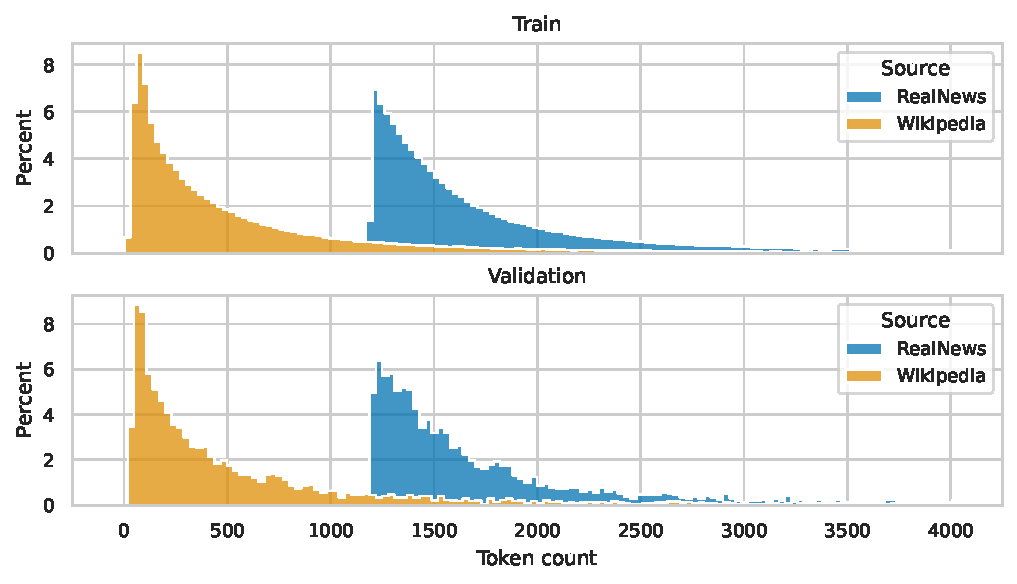
\includegraphics[width=\textwidth]{./img/val_data_dist.pdf}

  \caption{Distribution of train and validation documents' lengths for
  \Dataset{val-500k}.}

  \label{fig:val_data_dist}

\end{figure}

\section{Validation tasks}\label{section:validation_tasks}

We compare the embedding models based on their performance on downstream tasks.
We use a subset of our evaluation tasks, described in detail in
Chapter~\ref{chapter:evaluation}. We include tasks with either a large enough
training split suitable for cross-validation or a validation split. As a result, we validate embedding models only on classification tasks. All tasks are
evaluated using a validation split, except for \Task{IMDB}, where we take the
mean score of five cross-validation folds. To make the validation faster to
compute, we downsample the validation and train splits to 10000 examples. We
downsample the datasets following their label distribution so that the
truncated split has a label distribution nearly identical to the original one.
We present the validation tasks and their document count in
Table~\ref{table:validation_tasks}.

We use binary or micro-averaged accuracy as the scoring metric. Often, we compare
performance across several tasks. However, not all tasks are equally difficult,
so averaging accuracies would lead us to favor models that performed well on
easy tasks and undervalue models that performed well on more difficult tasks.
Therefore, we normalize the accuracy by the highest score reached for the given
task within the considered models, making the tasks equally difficult. We call
this metric \emph{normalized accuracy}. When more tasks are taken into account,
we asses models based on the mean normalized accuracy. In visualizations, we
mark mean normalized accuracy with a black triangle.

When validating a trained embedding model on a task, we finetune a head that
transforms the embeddings into the output format required by the given task. We
do not finetune the embedding model itself. Besides speeding up the validation,
this gives us a more genuine picture of the embedding model's performance.
Since all our validation tasks are classifications, we train a classification head for all of them. For each task, we use the same 2-layer neural network with a cross-entropy loss. We present the complete
list of the classifier's hyperparameters and training parameters in
Table~\ref{table:head_train_params}.

\begin{table}
  \footnotesize
  \centering
  \begin{tabular}{llrrrr}
    \toprule
      & \multicolumn{2}{c}{Documents} & Classes & \multicolumn{2}{c}{Class percentage} \\
    \cline{2-3} \cline{5-6}
      Dataset & Train & Validation & & Train & Validation \\
    \midrule
      \Task{arxiv} \citep{arxiv_papers} & \dag10 000 & 2 500 & 11 & 9.09$\pm$1.24\% & 9.09$\pm$1.01\% \\
      \Task{imdb} \citep{maas2011learning} & \dag10 000 & - & 2 & 50.00$\pm$0.00\% & - \\
      \Task{oc} \citep{zhou2020multilevel} & \dag10 000 & \dag10 000 & 2 & 50.00$\pm$0.06\% & 50.00$\pm$0.15\% \\
      \Task{aan} \citep{zhou2020multilevel} & \dag10 000 & \dag10 000 & 2 & 50.00$\pm$1.50\% & 50.00$\pm$4.57\% \\
      \Task{s2orc} \citep{zhou2020multilevel} & \dag10 000 & \dag10 000 & 2 & 50.00$\pm$0.09\% & 50.00$\pm$0.32\% \\
      \Task{pan} \citep{zhou2020multilevel} & \dag10 000 & 2 908 & 2 & 50.00$\pm$0.00\% & 50.00$\pm$0.00\% \\
    \bottomrule
  \end{tabular}

  \caption{Validation tasks we use to compare embedding models in this chapter.
  We truncated splits marked with {\dag} to speed up the evaluation process. We
  truncate a split by downsampling it following its label distribution. We also
  show the mean and standard deviation of class percentages to show all tasks
  have failry balanced class distributions.}

  \label{table:validation_tasks}

\end{table}


\begin{table}
  \centering
  \footnotesize

  \begin{tabular}{l c}
    \toprule
    Parameter & Value \\
    \midrule
    Hidden features & 50 \\
    Hidden dropout rate & 0.5 \\
    Hidden activation & ReLU \\
    Epochs & 10 \\
    Batch size & 32 \\
    Weight decay & 0.1 \\
    Label smoothing & 0.1 \\
    Learning rate & 1e-4 \\
    Learning rate decay & Cosine \\
    Maximum gradient norm & 1.0 \\
    Optimizer & AdamW \\
    Mixed-precision training & Yes \\
    \bottomrule
  \end{tabular}

  \caption{Hyperparameters used for training classification heads during
  evaluation in this chapter.}

  \label{table:head_train_params}

\end{table}

\section{Student model's configuration and baselines}\label{section:student_model_config_baselines}

As we explain in Section~\ref{section:student_model}, we initialize our
student model with Longformer \citep{beltagy2020longformer}. We use
Longformer's base version with about 126M parameters implemented by HuggingFace
\texttt{transformers}
library\footnote{\url{https://huggingface.co/allenai/longformer-base-4096}}.

We generate the student's embedding by computing a mean of the last layer's hidden states. We do not use global attention and employ sliding window
attention, with the window sizes $\omega$ set to the default 512 tokens. In our
preliminary experiments, we also tested setting global attention to the
\texttt{CLS} token and taking its hidden state from the last layer as the
input's embedding. However, the mean-pooling approach proved to be superior.
Additionally, with mean-pooling, we found global attention is not beneficial,
so we do not use it.

During training, we aim for fast convergence with a small memory footprint. Therefore, we use a high learning rate, no gradient
accumulation steps, mixed-precision training, and gradient checkpointing. We
enumerate the complete list of student's training parameters in
Table~\ref{table:student_train_params}. We use these values for all students
we train in this chapter.


\begin{table}
  \centering
  \footnotesize

  \begin{tabular}{l c}
    \toprule
    Parameter & Value \\
    \midrule
    Batch size & 6 \\
    Weight decay & 0.1 \\
    Learning rate & 1e-4 \\
    Learning rate decay & Cosine \\
    Maximum gradient norm & 1.0 \\
    Optimizer & AdamW \\
    Gradient accumulation steps & 1 \\
    Warmup steps & 10\% of training steps \\
    Gradient checkpointing & Yes \\
    Mixed-precision training & Yes \\
    \bottomrule
  \end{tabular}

  \caption{Training parameters' values we use every time we train a student model in this chapter.}

  \label{table:student_train_params}

\end{table}

\subsection{Baselines}

As mentioned, our goal is to find a configuration of our training method such that the trained student outperforms both teachers and Longformer. To check how close we are to this goal
throughout this chapter, we compare the students to three models:
Longformer \citep{beltagy2020longformer}, SBERT \citep{reimers2019sentence},
and PV \citep{le2014distributed}. We compare students to Longformer to judge how our training method improves document embeddings. Due to the selection of our training data, the student's performance depends only on our training method. Thus, the student model's performance becomes proportional to our training method's performance. As we also want to consume a minimum amount of resources, we train the student models only on 15k documents. In our preliminary experiments, we found this number of training documents to be enough to show the benefit of our method. For context, we train the student models for only 3.8\% of Longformer's pre-training iterations with an eight times smaller batch size.

We compare the students to the two teachers to see how much performance our
training method ignores or takes advantage of. If our student model performs
worse than a particular teacher, we need to improve how we distill the
teacher's embeddings into the student's embeddings. As the student has
architectural advantages compared to both teachers, such as longer maximum
context, we hypothesize it can match and surpass both teachers' performance. We
discuss the configuration of the structural teacher in the following section. We train Paragraph Vector as a part of our method in Section~\ref{section:pv_training}.

\section{Structural loss}\label{section:structural_loss}

We start our experiments with the structural loss $\Loss_S$. The structural
loss compares the student's and the structural teacher's embeddings. Its
goal is to encourage distillation of the quality of the structural teacher's
embeddings into the student's embeddings. We focus on the structural loss first
since, in our preliminary experiments, we observed that the structural quality
is more important to the performance of the student model than the contextual
quality. We arrive at the same conclusions later in this chapter in
Section~\ref{section:projections_only_contextual}. Therefore, we prioritize first finding the best-performing hyperparameters of the structural loss and
adapting the contextual loss to it afterward.

As we mention in Section~\ref{section:teacher_models}, we use SBERT
\citep{reimers2019sentence} as our structural teacher. We use SBERT's version
initialized with MPNet \citep{song2020mpnet} since it is a relatively small
model with above-average
performance\footnote{\url{https://sbert.net/docs/pretrained_models.html}}. We
use SBERT's implementation from the HuggingFace \texttt{transformers}
library\footnote{\url{https://huggingface.co/sentence-transformers/all-mpnet-base-v2}}
with a mean pooling layer above the last layer's hidden states. We do not
perform any finetuning and use the pre-trained weights only.

As explained in Section~\ref{section:abstract_loss}, we choose structural loss
to be more restrictive, forcing an exact similarity between the two embeddings.
Therefore, we test two different exact losses as structural losses: Mean Squared
Error (\emph{MSE}) and cosine distance. We try MSE because it forces
equality, the most restrictive similarity measure. The motivation for using
cosine comes from the embeddings' use cases, where cosine distance is a popular
similarity measure. More importantly, it is also used by SBERT's authors,
suggesting that for SBERT's embeddings, it is the best-performing similarity
measure.

We train the student model with each loss on the first 15k documents of
\Dataset{val-500k} with the hyperparameters given in
Section~\ref{section:student_model_config_baselines}. As we show in
Figure~\ref{fig:structural_basic}, with cosine distance, the student model
surpasses both baselines. The fact that the student performs better
than the teacher indicates that Longformer's longer context and supervision from
the structural teacher can boost the student's performance even above the level
of the teacher. Moreover, SBERT's scores are significantly higher than
Longformer's, showing that unless Longformer's embeddings are finetuned, its
longer context length or pre-training is of no benefit.

These encouraging results show that using only the structural teacher can be a
valid method of improving a model's embeddings in itself, even without the contextual teacher. In subsequent experiments, we
use cosine as the structural loss. For brevity, we label the student model
trained with only the cosine structural loss as \Model{only-structural;cosine}.

\begin{figure}
  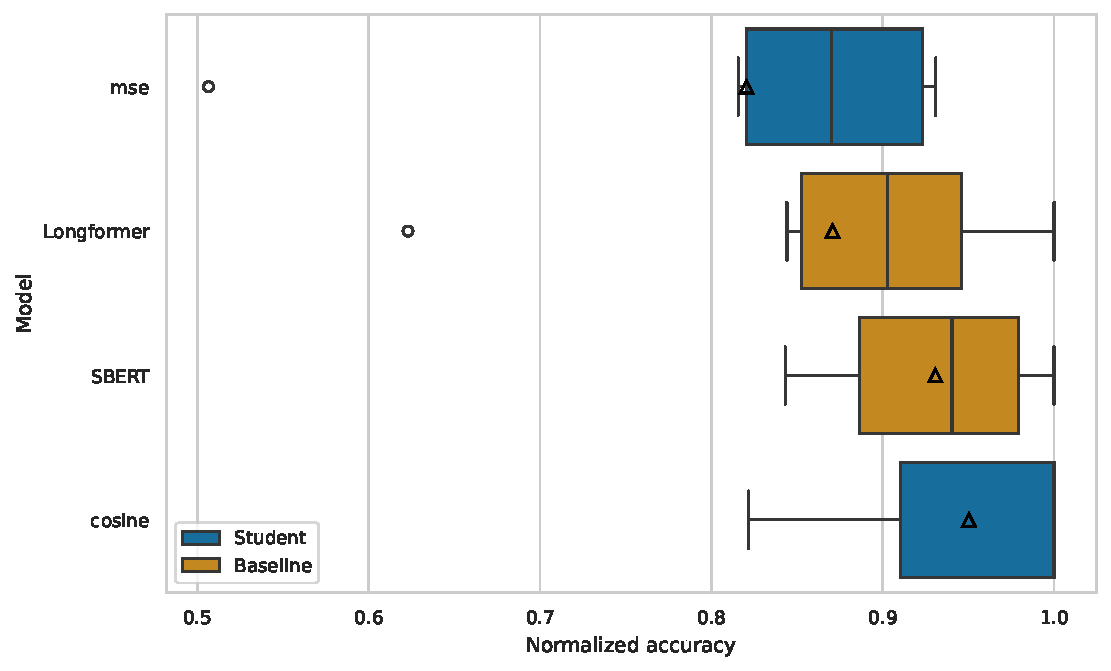
\includegraphics[width=\textwidth]{img/structural_simple_losses.pdf}

  \caption{Performance of student models trained with only the structural
  teacher.}

  \label{fig:structural_basic}
\end{figure}

\subsection{Composite structural losses}\label{section:composite_losses}

Besides the cosine and the MSE, we also explore losses that combine a positive
and a negative component, such as contrastive loss. We call these losses
\emph{composite} to differentiate them from \emph{simple} losses, such as MSE or cosine
distance. Composite losses compare the student's embedding to a teacher's
embedding of the same input, which we call \emph{positive}, and to
the teacher's embedding of different inputs, which we call
\emph{negatives}. They reward the student model for close proximity to
positives or large distances to the negatives. Therefore, structural composite
losses aim to optimize two objectives: they decrease the distance to SBERT's embeddings
while increasing the margin between the student's embeddings of different inputs.

We explore two types of composite losses: max-margin and contrastive. To
formulate these losses, we label the student's embedding as $y$, the
corresponding teacher's embedding as $y_{\text{pos}}$, the set of negatives as
$Y_{\text{neg}}$, the given similarity measure as $\operatorname{sim}$, and a
weighting parameter as $\gamma$. We define the max-margin loss in
Equation~\ref{eq:max_marginals} and the contrastive loss in
Equation~\ref{eq:contrastive}.

\begin{equation}
  \Loss_{\text{max-margin}}(y, y_\text{pos}, Y_\text{neg}) =
    \operatorname{sim}(y, y_\text{pos}) -
    \gamma \frac{1}{|Y_\text{neg}|} \sum_{y_\text{neg} \in Y_\text{neg}}
      \operatorname{sim}(y, y_\text{neg})
  \label{eq:max_marginals}
\end{equation}

\begin{equation}
  \Loss_{\text{contrastive}}(y, y_\text{pos}, Y_\text{neg}) =
    -\log \frac{
      \exp(\cos(y, y_\text{pos}))
    }{
      \exp(
        \cos(y, y_\text{pos}) +
        \sum_{y_\text{neg} \in Y_\text{neg}} \cos(y, y_\text{neg})
      )
    }
  \label{eq:contrastive}
\end{equation}

For max-margin loss, we try MSE and cosine distance as $\operatorname{sim}$ and
simultaneously try several weightings $\gamma$. We compare models trained with
the composite losses with those trained with the simple losses in
Figure~\ref{fig:structural_composite_vs_simple}. Composite losses using MSE
seem to benefit from the negative loss component, as 3 out of the 4 tested outperform the
simple MSE loss. However, despite the benefits, only one variant surpasses both
baselines. With cosine, it seems that the negative loss component hurts the
performance since only one version outperforms the simple cosine loss and does
so by only $10^{-4}$. We carry out an analysis to explain the differences
between MSE and cosine composite losses and to show how the negatives
contribute to the model's performance.

\begin{figure}

  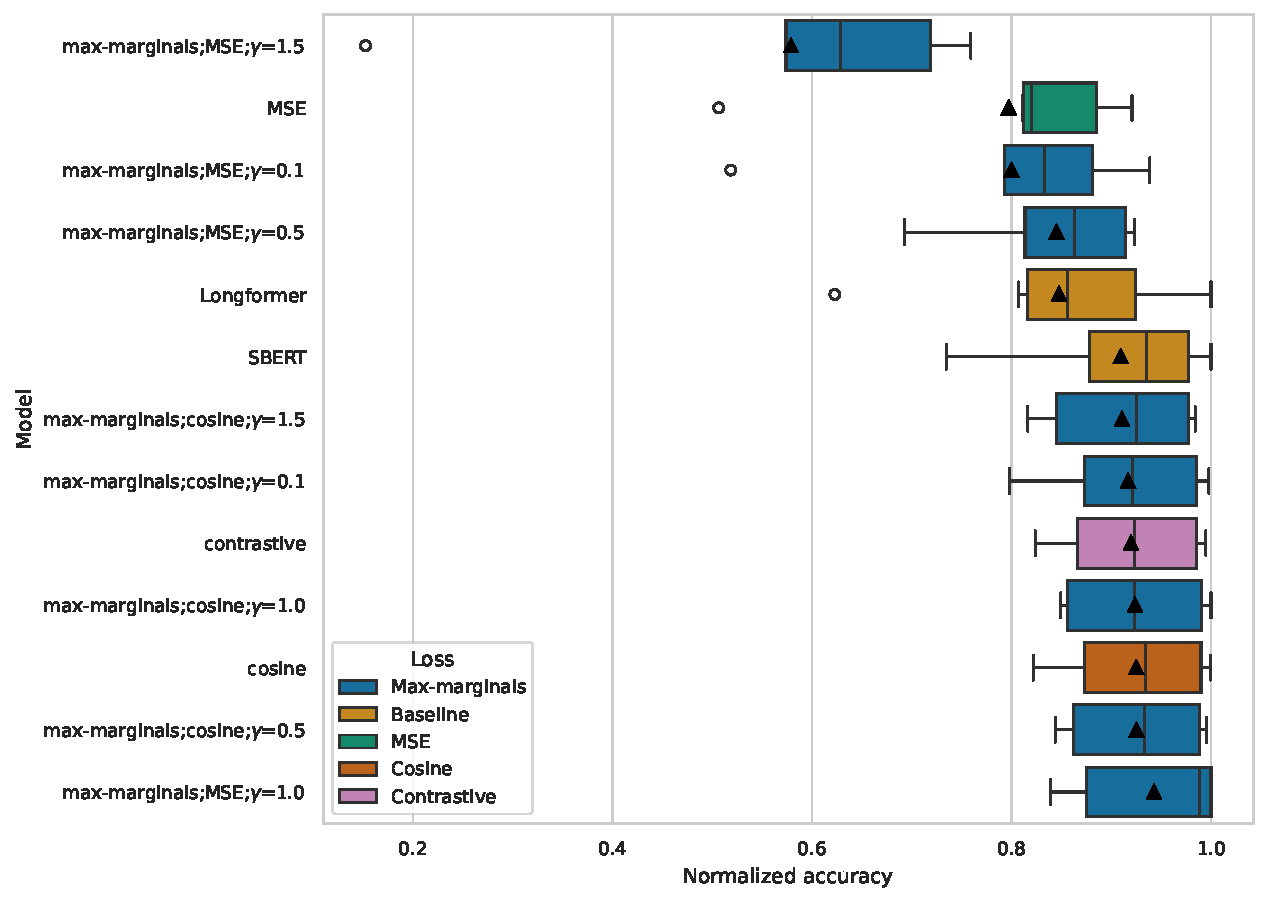
\includegraphics[width=\textwidth]{./img/structural_both_losses.pdf}

  \caption{Performance of student models trained with composite and simple
  structural losses.}

  \label{fig:structural_composite_vs_simple}
\end{figure}

\subsubsection{Analysis of composite losses}\label{section:composite_analysis}

The impact of composite losses is different for MSE and cosine. Also, it is not
clear how the negatives contribute to the student's performance. To explain
these results, we compare the distances to positives and negatives for several
chosen models in Figure~\ref{fig:composite_distances}. The plotted distances
nicely mirror the students' performances. However, the effect of the negative
loss component is minimal for most student models. Except for
\Model{max-margin;MSE} with $\gamma$ set to 1 or 1.5, there is no dramatic
shift in the distances' distributions. In terms of squared L2 distance,
\Model{max-margin;MSE;$\gamma$=1.0} widens the gap between positives and
negatives, yet it also increases the distances to the positives. However, this
effect is much less pronounced for cosine distance. This suggests that the model increases the
embeddings' norm to create a large gap between positives and negatives in terms
of squared L2 distance while decreasing the cosine distance to positives. In
other words, despite computing L2 distances, max-margin MSE loss with
$\gamma=1.0$ optimizes cosine distance. Note that with $\gamma=1.5$, the
negative loss component has damaging effects in terms of both cosine and
squared L2 distances.

\begin{figure}
  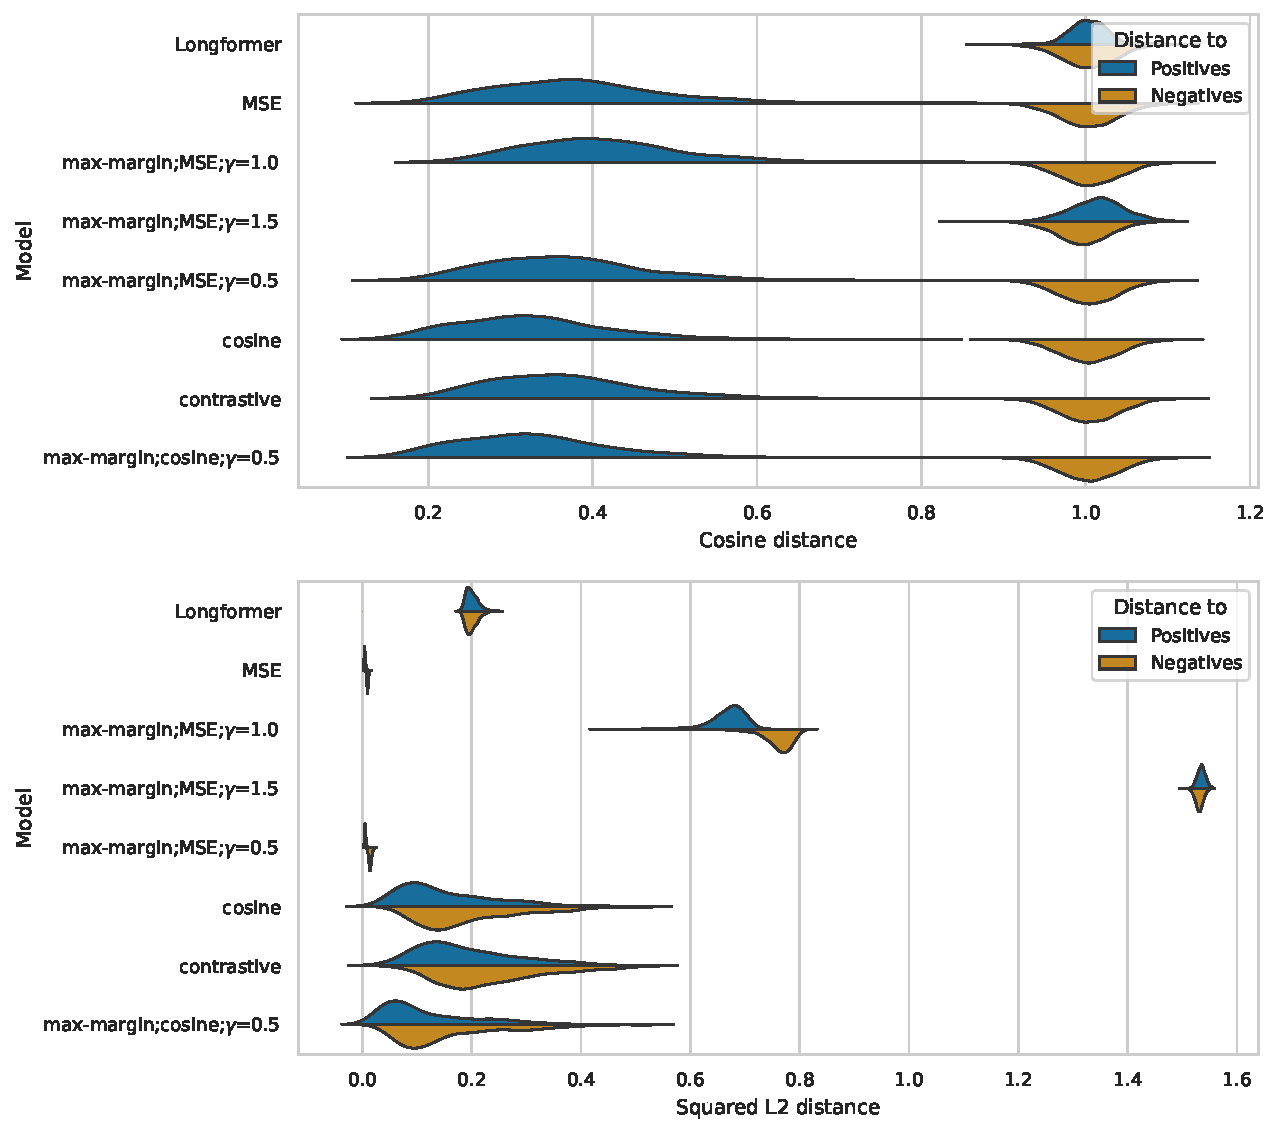
\includegraphics[width=\textwidth]{img/composite_distances.pdf}

  \caption{Distribution of distances between the model's and the structural
  teacher's embeddings. A distance to the teacher's embedding of the same
  document is labeled as \emph{positive}, whereas distances to the teacher's
  embedding of another document are labeled as \emph{negative}. We generated
  the distances from the first 1000 documents of \Dataset{val-500k}'s
  validation split.}

  \label{fig:composite_distances}

\end{figure}

To summarize, the effect of the negatives being included in the loss may be
dual. With the right configuration, the composite losses may enforce a larger
separation between the student's embeddings while decreasing their
distance from the structural teacher's embeddings. So, besides
\Model{only-structural;cosine} we also continue experimenting with
\Model{max-margin;MSE;$\gamma$=1.0}, which we label in further sections as
\Model{only-structural;mm-MSE}.

\section{Structural and contextual loss}\label{section:structural_and_contextual}

This section explores contextual losses to complement the best-performing
structural losses from the previous section. Since there are several
hyperparameters to explore, we split this section into parts. Each part focuses
on a different aspect of the contextual loss or the weighting of the contextual
and structural loss. At the end of each part, we select a few best-performing
variants, which serve as a starting point in the subsequent section. First, we
test different training hyperparameters of the contextual teacher in
Section~\ref{section:pv_training}. Then, we experiment with the contextual
loss's configuration in Section~\ref{section:contextual_loss}. To illustrate
the importance of the structural teacher, we show the performance we reach when
we use only the contextual loss. More importantly, we test the contextual
losses with both selected structural losses and pick the best-performing configuration
for each one. Finally, we explore different ways to weigh the contextual and
structural loss for both combinations in
Section~\ref{section:weighting_experiments}.

\subsection{Optimizing Paragraph Vector's training}\label{section:pv_training}

We choose Paragraph Vector \citep{le2014distributed} as our contextual teacher,
as we elaborate on in Section~\ref{section:paragraph_vector}. Since there is no
concept of a pre-trained PV, as in the case of Transformers, we train PV from
scratch. We use PV's implementation from the Gensim
library\footnote{\label{fn:link_to_gensim}\url{https://radimrehurek.com/gensim}}
and explore some of the hyperparameters that govern the training of PV. We
focus on four hyperparameters that we consider important and adopt the
recommendation of the library or related literature for the rest of them. We enumerate the adopted
and the grid-searched hyperparameters in Table~\ref{table:pv_hyperparams}. To
explain the meaning of all hyperparameters, we provide the following summary:


\begin{itemize}

  \item \texttt{dm} --  PV architecture; true for Distributed Memory (DM),
    false for Distributed Bag of Words (DBOW)

  \item \texttt{vector\_size} -- dimensionality of the generated embedding

  \item \texttt{min\_count} -- words with document frequency below this limit
    will be ignored

  \item \texttt{text\_pre\_process} -- applied word processing done before the
    model's training; for stemming, we use PorterStemmer implemented by the \texttt{nltk}
    library\footnote{\url{https://www.nltk.org/api/nltk.stem.porter.html}}

  \item \texttt{negative} -- number of noise words used for negative sampling
    during training

  \item \texttt{window} -- the maximum distance between known and predicated
    word

  \item \texttt{sample} -- percentile threshold configuring which words will be
    downsampled; 0 for no downsampling


  \item \texttt{dbow\_words} -- whether to train word embeddings using
    Word2Vec's \citep{mikolov2013efficient} Skip-gram architecture together
    with document embeddings; only applicable to DBOW, as DM learns word embeddings by default

  \item \texttt{epochs} -- a number of iterations done over the corpus during
    training

\end{itemize}


As recommended by the authors of PV \citep{le2014distributed}, we experiment
with both architectures. For each architecture, we try different values of
\texttt{vector\_size}, \texttt{min\_count}, and \texttt{text\_pre\_process},
which all control the model's regularization. Settings such as higher
dimensional embedding, small minimum count, and no text pre-processing
regularize the model the least. They give the model the most information on its
inputs while providing it with a large embedding through which it
can express precisely. On the other hand, using lower dimensional embedding,
large minimum count, and stemming forces the model to be
more general and less precise. The model has less detailed information on its
input and must squeeze all of it into a small vector. We do not see any value in
trying dimensions of embeddings higher than 1024 since, in later experiments, we
must distill the contextual embedding to a 768-dimensional embedding of our
student model. Intuitively, the larger the contextual embedding will be,
the smaller the fraction of information the student model will be able
to digest. Also, there is no value in considering \texttt{min\_count} to be
lower than two since we would only add words unique to a single
document. Embeddings of such words would be poorly trained and not add
meaningful information to the document's embedding. The last hyperparameter that is
worth mentioning is \texttt{dbow\_words}. DBOW, on its own, does not train word
embeddings, which are, by default, randomly generated. Setting \texttt{dbow\_words} to true
causes DBOW to train word embeddings using Word2Vec's Skip-gram model
\citep{mikolov2013efficient} in each epoch. \cite{lau2016empirical} showed that
random word embeddings significantly hurt the model. Consequently, when
training DBOW, we also train word embeddings despite the slower training, which
it inevitably causes.

\begin{table}
  \footnotesize
  \centering
  \begin{tabular}{lrc}
    \toprule
    Hyperparameter & Value(s) & Recommended by \\
    \midrule
    \texttt{dm} & true, false & - \\
    \texttt{vector\_size} & 100, 768, 1024 & - \\
    \texttt{min\_count} & 2, 10\% of training corpus& - \\
    \texttt{text\_pre\_process} & stem, lowercase, none & - \\
    \texttt{window} & 5 & default \\
    \texttt{negative} & 5 & default, \cite{lau2016empirical} \\
    \texttt{sample} & 0 & default \\
    \texttt{dbow\_words} & true & \cite{lau2016empirical} \\
    \texttt{epochs} & 10 & default, \cite{dai2015document} \\
    \bottomrule
  \end{tabular}

  \caption{Used hyperparameters for training Paragraph Vector. We grid-searched
  four hyperparameters: PV architecture, vector size, minimum word count, and
  pre-processing of words. For the rest of the hyperparameters, we adopted either the
  default values or recommended by the mentioned literature.}

  \label{table:pv_hyperparams}

\end{table}

We train all variants on the whole \Dataset{val-500k} corpus. We follow the
recommendations of \cite{le2014distributed} and also evaluate the combination
of both architectures. However, we only select the best three models from each
architecture and evaluate all nine combinations. We call these models
\emph{compound} Paragraph Vectors. We evaluate 45 models and display their
performance on validation tasks in Figure~\ref{fig:pv_val_scores}.
The single models favor large embedding dimensions and low minimum count.
Additionally, on average, stemming or lowercasing leads to higher scores than
not pre-processing the words. DBOWs vary more in performance, occupying the
best and the worst positions, whereas DMs are more consistent. We achieve a
slight improvement by concatenating a DM and a DBOW model, but considering the
resulting model has an embedding twice as large, the improvement is not
surprising. Interestingly, all compound models perform very similarly,
suggesting that slight imperfections of one model can be compensated by another
model of a different architecture.

\begin{figure}

    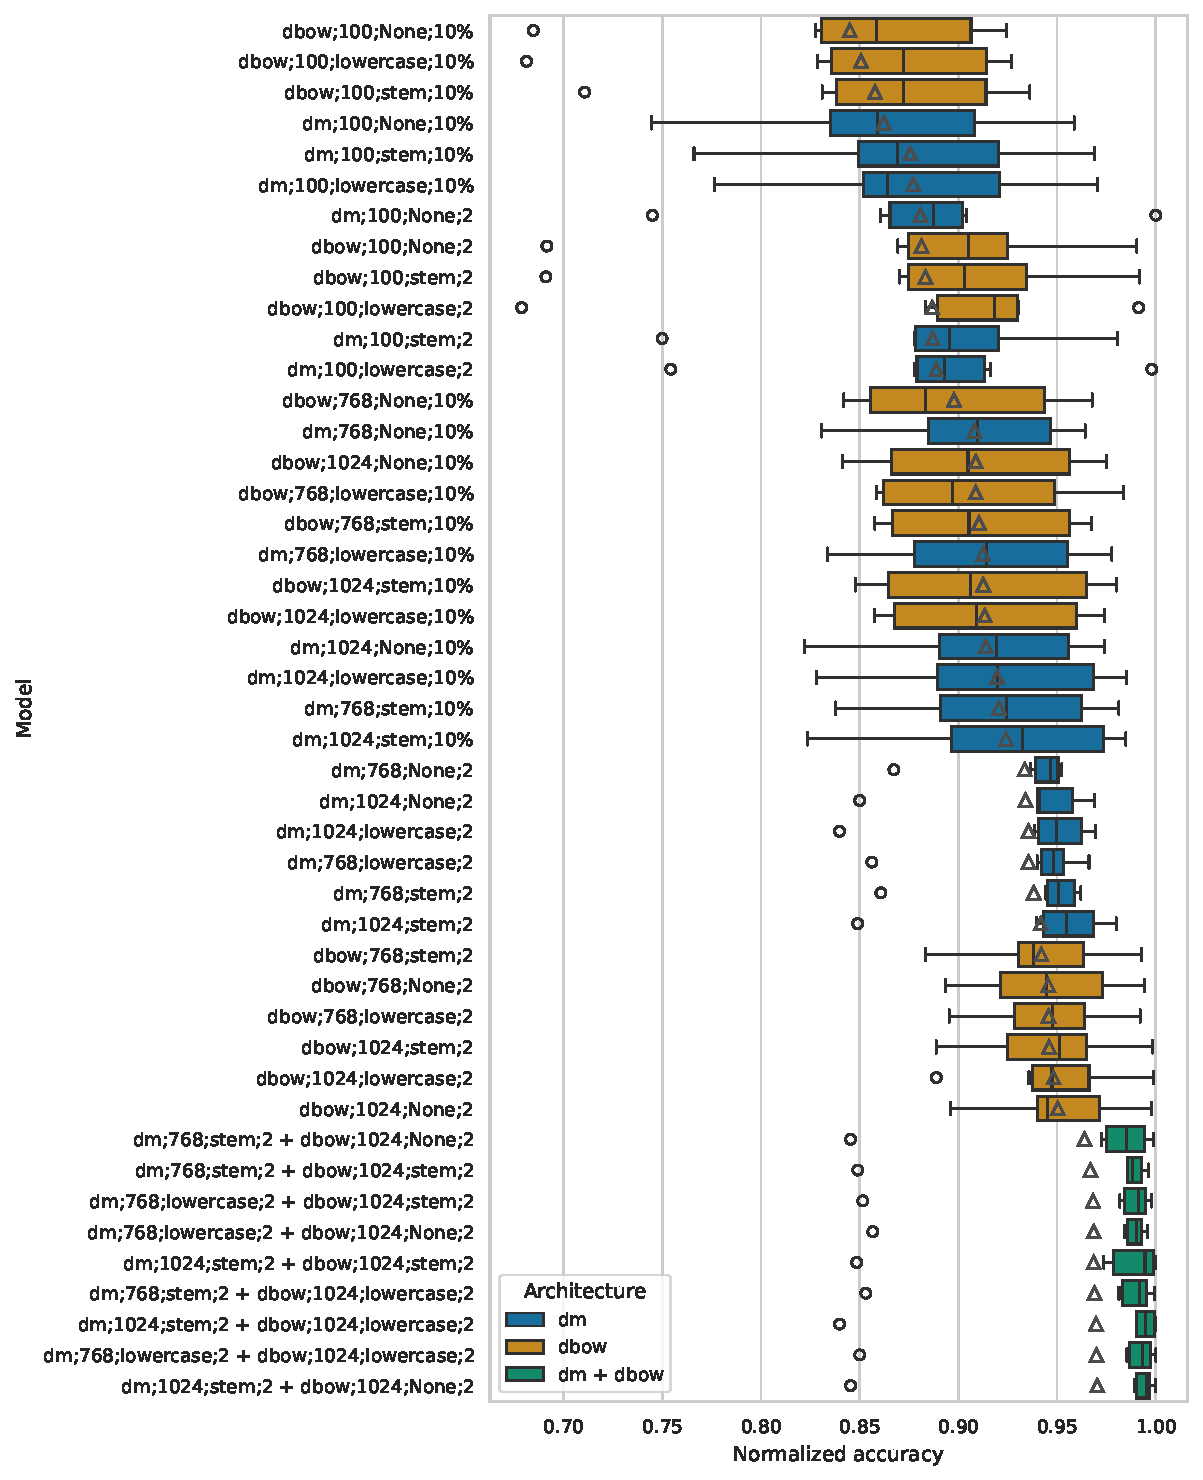
\includegraphics[width=\textwidth]{./img/pv_val_scores.pdf}

    \caption{Performance of all Paragraph Vector variants on validation tasks.
    We identify a model by its architecture, embedding dimension, text
    pre-processing, and minimum count. Compound models are identified as a
    concatenation of such identifiers separated by $+$.}

    \label{fig:pv_val_scores}

\end{figure}

In our preliminary experiments, we saw that the dimension of contextual teacher
embedding plays a significant role in teacher-student training. So, we select
three paragraph vectors with varying vector sizes. We pick the best model with
small vector size (\Model{DM;100;lowercase;2}), the best single model
(\Model{DBOW;1024;None;2}) and the best model composed of both architectures
(\Model{DM;1024;stem;2+DBOW;1024;None;2}). For brevity, we label these models as
\Model{DM;100d}, \Model{DBOW;1024d} and \Model{PV;2048d} respectively.

\subsection{Contextual loss}\label{section:contextual_loss}

Contextual loss $\Loss_C$ compares the student's and the contextual teacher's
embeddings and encourages distillation of the quality of the teacher's
embedding into the student's embedding. As we discuss in
Section~\ref{section:abstract_loss}, we choose $\Loss_C$ to be less strict and
give the student model more freedom in encoding the input into the
document embedding. Consequently, we do not consider losses such as MSE or
cosine since they enforce either an exact vector or a direction in the
embedding space. Instead, we use a variant of \emph{Canonical Correlation
Analysis} \citep{hotelling1992relations} (\emph{CCA}). In its base form, CCA
computes a correlation of two linearly projected sets of vectors, where the
projections are optimized to maximize the correlation. We define CCA
in Equation~\ref{def:cca_more_dim}.

\begin{defn}[Canonical Correlation Analysis]\label{def:cca_more_dim}

  For two matrices $X_1 \in \mathbb{R}^{n_1 \times m_1}$ and $X_2 \in
  \mathbb{R}^{n_2 \times m_2}$, Canonical Correlation Analysis for $k$
  dimensions finds $P \in \mathbb{R}^{m_1 \times k}$ and $Q \in \mathbb{R}^{m_2
  \times k}$ that maximize

  \begin{equation}
    \begin{split}
      &\CCA(X_1, X_2) = \sum_{i = 1}^k \corr(X_1P_{*i}, X_2Q_{*i}) \\
      \text{s.t.}\quad &P^TX_1^TX_1P = I_k = Q^TX_2^TX_2Q \\
    \end{split}
  \end{equation}


\end{defn}

CCA gives the student the freedom to change its embeddings as long as their
linear projections correlate more with the linear projections of the contextual
teacher's embeddings. However, linear projection may still leave too little
leeway for the student model to mimic the structural teacher. Ideally, we would like to regulate the strength of the projections. Such adjustment is possible with \emph{Deep CCA} (\emph{DCCA})
\citep{andrew2013deep}. DCCA projects the input vectors with two neural
networks and feeds the projections to the vanilla CCA. The two networks are
trained jointly with the embedding model based on the computed CCA, which is
used as a loss. The advantage of DCCA is that we can adjust the strength of the
projections and thereby regulate the pressure the contextual loss inflicts on
the student model. The larger the neural network is, the more it can transform
the embeddings and the less the student model needs to adjust its embedding.

As we can see in Equation~\ref{def:cca_more_dim}, CCA is computed from the
entire dataset of input vectors. And so DCCA is trained using a full-batch
optimization \citep{andrew2013deep} or a mini-batch optimization with large
batch sizes \citep{wang2015unsupervised}. However, both methods need large
amounts of GPU memory and are suitable only with smaller models. For this
reason, we avoid CCA and use SoftCCA \citep{chang2018scalable} instead. SoftCCA
reformulates CCA such that it is usable even in the case of mini-batch
optimization with small batches. To explain how SoftCCA is related to CCA, we
reformulate the solution to CCA using a Forbenious matrix norm in
Equations~\ref{def:cca_with_forbenious_first}-\ref{def:cca_with_forbenious_last}.

\begin{align}
  P^\ast, Q^\ast &= \underset{P, Q}{\argmin} ||X_1P - X_2Q||^2_F \label{def:cca_with_forbenious_first} \\
  &= \underset{P, Q}{\argmin} \trace\left((X_1P - X_2Q)^T(X_1P - X_2Q)\right) \\
  &= \underset{P, Q}{\argmin} {-2} \trace(P^TX_1^TX_2Q) \\
  &= \underset{P, Q}{\argmax} \trace(P^TX_1^TX_2Q) \\
  &= \underset{P, Q}{\argmax} \sum_{i = 1}^k \corr(X_1P_{*i}, X_2Q_{*i}) \label{def:cca_with_forbenious_last}
\end{align}

Thus, by minimizing CCA, we effectively minimize the difference between two
projections with uncorrelated features. SoftCCA enforces the same behavior
with two separate losses:

\begin{itemize}

  \item L2 loss, which minimizes the difference between a projected set of
    vectors $Z_1$ and $Z_2$:

    \begin{equation}
      \Loss_{\text{L2}}(Z_1, Z_2) = ||Z_1 - Z_2||^2_F = \MSE(Z_1, Z_2)
    \end{equation}

  \item \emph{Soft Decorrelation Loss} (\emph{SDL}), which forces a projected
    set of vectors $Z$ to have decorrelated features:

    \begin{equation}
      \Loss_{\text{SDL}}(Z^t) = \sum_{i \ne j} \left|
          \frac{(\Phi^t_Z)_{ij}}{\hat{\beta}^t}
          \right|
    \end{equation}
    where
    \begin{align}
      \Phi^t_Z &= \beta \Phi^{t-1}_Z + \Sigma_{Z^t} \\
      \Phi^0_Z &= \bm{0}_d \\
      \hat{\beta}^t &= \beta \hat{\beta}^{t-1} + 1 \\
      \hat{\beta}^0 &= 0
    \end{align}

\end{itemize}

Where the symbols above have the following meanings:

\begin{itemize}

  \item $Z, Z_1, Z_2 \in \mathbb{R}^{b \times d}$ are mini-batches of
    $d$-dimensional vectors

  \item $\Sigma_{Z}$ is a covariance matrix of a mini-batch of vectors $Z$

  \item $\bm{0}_d$ is a $d \times d$ zero matrix

  \item $\beta$ is a hyperparameter

  \item $\Phi_Z^t, Z^t, \hat{\beta}^t$ is $\Phi_Z, Z, \hat{\beta}$ at iteration
    $t$

\end{itemize}

The L2 loss forces the projected vectors to be equal, while the Soft
Decorrelation Loss forces them to have uncorrelated features. SoftCCA can approximate CCA by keeping a running mean of the projected vectors' covariance matrices. Similarly to Batch Normalization \citep{ioffe2015batch},
SDL updates the running mean during training but avoids any updates during
inference. With the above losses and the weighting hyperparameter $\delta$, we
define SoftCCA in Equation~\ref{eq:soft_cca}.

\begin{equation}\label{eq:soft_cca}
  \Loss_{\text{SoftCCA}}(Z_1, Z_2) = \Loss_{\text{L2}}(Z_1, Z_2) +
      \delta ( \Loss_{\text{SDL}}(Z_1) + \Loss_{\text{SDL}}(Z_2) )
\end{equation}

We use SoftCCA loss as a replacement for CCA in DCCA. To be explicit, we
project the student's and the contextual teacher's embedding with two separate
feed-forward neural networks. Then, we apply SoftCCA loss, which provides a
training signal for the embedding model and the neural networks projecting the
embeddings. Depending on which input the neural networks project, we call them
\emph{student} and \emph{contextual projections}. And so, we can finally express $\Loss_C$ from
Equation~\ref{eq:abstract_loss} more concretely. For a student projection
$f_\Student$ and a contextual projection $f_C$, we formulate our contextual
loss in Equation~\ref{eq:contextual_loss}. We also illustrate the architecture
of contextual loss graphically in Figure~\ref{fig:contextual_loss}.

\begin{equation}\label{eq:contextual_loss}
  \Loss_C(y_\Student, y_{\Teacher_C}) = \Loss_{\text{SoftCCA}}(
    f_\Student(y_\Student),
    f_C(y_{\Teacher_C})
  )
\end{equation}

\begin{figure}

  \centering
  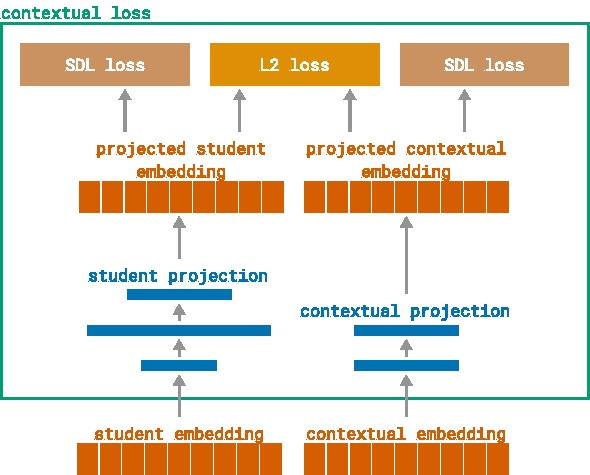
\includegraphics[width=0.7\textwidth]{img/contextual_loss.pdf}

  \caption{Architecture of contextual loss.}

  \label{fig:contextual_loss}

\end{figure}

In our preliminary experiments, we found that the value of $\delta$ from
Equation~\ref{eq:soft_cca} has little effect on the final student's
performance. So, we set it so that the ranges of $\Loss_{\text{L2}}$ and
$\Loss_{\text{SDL}}$ are roughly equal. On the other hand, choosing the right
value of $\beta$ proved to be critical. Based on how the CCA of the projected
embeddings of the validation split progressed throughout the training, we found
the optimal value to be 0.95, which puts a relatively large emphasis on the
accumulated mean compared to lower values of $\beta$.

In the rest of this section, we experiment with the strength of the
projections. In the following section, we build the basic intuition behind
training with contextual loss while finding the ideal projections without
structural loss. In the subsequent sections, we study how different
structural losses influence the projections. First, we experiment with cosine
and then with max-margin MSE loss. In all cases, we test the projections for
each of the three contextual teachers: \Model{DM;100d}, \Model{DBOW;1024d} and
\Model{PV;2048d}. Finally, we select the best contextual loss with the best
contextual teacher for both cosine and max-margin MSE structural loss.

\subsubsection{Contextual projection with contextual loss
only}\label{section:projections_only_contextual}

With only the contextual loss, the student's only goal is to mimic the
contextual teacher. This presents an elementary setting in which we can study
the behavior of the projections and the contextual loss as a whole without
any influence from the structural loss.

Our preliminary experiments show that the projections' over-parameterization
hurts the model's performance. Even though large projections result in smaller
SoftCCA loss, they tend to harm the CCA computed on the student's and
contextual teacher's embeddings. Strong projections compensate for the
student's flaws, lessening the pressure on the student model as it does not
need to adjust its embedding much. Consequently, the student model learns very
little compared to the projections. Similarly, strong contextual projection
takes away pressure from the student projection and vice-versa. In this regard,
it is essential to keep the contextual projection small. This puts more
pressure on the student's side, where the gradients can propagate to the
embedding model.

As we mentioned before, we feed the projected outputs to SoftCCA loss
$\Loss_{\text{SoftCCA}}$. SoftCCA requires both inputs to be of the same
dimension, so both projections must end with an equally sized layer. We always use
the dimension of the larger embedding as the final projection dimension. We do
so to preserve all the embeddings' information through the projection and force
the student model to distill all the contextual embedding's dimensions, not just
their subset. Also, there is no point in projecting the embeddings to even more
dimensions than the embeddings have. Due to the Pigeonhole principle, some
features of the final projections would have to depend on the same embedding's
features and, therefore, would correlate with each other. Such correlations
would create unnecessary conflict with the SDL loss. This phenomenon would also
occur for projections with an hourglass shape, where there is one bottle-neck
layer with significantly fewer dimensions than the layers after or before it.
And indeed, during preliminary testing, we saw these projections always perform
poorly.

We build the projections as a sequence of blocks, where each block is composed
of a fully connected layer and an optional Rectified Linear Unit (\emph{ReLU}).
In preliminary experiments, we also tried adding Dropout, Batch, or Layer
Normalization layers at different places in a block. However, in all cases,
they had either negligible or negative effects on the performance of the final
model. We label each block with the dimension of the fully connected layer and the activation's name in brackets if used. We identify a projection by
block's labels delimited by an ``x''. So, \Proj{768(ReLU)x1024} are two
feed-forward layers with 768 and 1024 features connected via ReLU. To label
projections without any layers, we use a dash. We present all the projections'
variations we tested in Table~\ref{table:contextual_projections}. Considering
the conditions described in the previous paragraph, we choose a strong and a
weak projection for both the student and contextual side. We are careful not to
over-parametrize either projection and lean toward stronger student projection.

\begin{table}
  \centering
  \footnotesize

  \begin{tabular}{lrrr}
    \toprule
      & \multicolumn{3}{c}{Contextual teacher's embedding dimension} \\
      \cline{2-4} \\
      Projection & 100 & 1024 & 2048 \\
    \midrule
      \multirow[t]{2}*{Student} & \TableProj{768(ReLU)x1024(ReLU)x768} & \TableProj{768(ReLU)x1024} & \TableProj{1024(ReLU)x2048} \\
      & \TableProj{768} & \TableProj{1024} & \TableProj{2048} \\
      \multirow[t]{3}*{Contextual} & \TableProj{100(ReLU)x768} & \TableProj{768x1024} & \TableProj{1024x2048} \\
      & \TableProj{768} & \TableProj{1024} & \TableProj{2048} \\
      & & - & - \\
    \bottomrule
  \end{tabular}

  \caption{All tested variants of projections with only contextual loss. We do
  a grid search of the given variants for each contextual teacher. This results
  in 16 combinations overall.}

  \label{table:contextual_projections}
\end{table}

We train the student models on the first 15k documents of \Dataset{val-500k}
and compare the models' performance to all the relevant teachers, Longformer
and \Model{only-structural;cosine} in Figure~\ref{fig:projections_contextual}.
We identify a student model with the contextual teacher's dimension, the
student projection prefixed by \Model{S:} and the contextual projection
prefixed by \Model{C:}.

The results correspond to those we witnessed in our preliminary experiments and
showcase some of the mentioned projections' behaviors. The better half of the
student models differs from the rest by having a minimal contextual projection.
Moreover, for a given contextual teacher and a projection, the student model
with a larger student projection outperforms the student with a smaller one in
all cases but one.

Half of the tested projections improve the score of Longformer. The better
projections demonstrate that we can distill useful information from the
contextual teacher to the student, while the worse projections highlight how
important the projections are. However, as our contextual loss does not enforce
an exact similarity of the student's and the contextual teacher's embedding,
most students do not outperform their respective contextual teachers.
Interestingly, students trained with \Model{DM;100d} surpass students trained
with better performing \Model{DBOW;1024d}. We can observe the same performance
differences for \Model{DBOW;1024d} and \Model{PV;2048d}, even if we compare
projections that scale with the contextual embedding, such as
\Proj{1024d;S:1024;C:-} and \Proj{2048d;S:2048;C:-} or
\Proj{1024d;S:1024;C:1024} and \Proj{2048d;S:2048;C:2048}. Consequently,
distilling information from an embedding with fewer features seems easier than
from a larger one. And so, even though PV with 2048 dimensions beats SBERT, the
students trained with it fail to capitalize on this advantage and perform worse than the model trained with SBERT. So, according to our results, the structural teacher is more important to the student's performance
than the contextual teacher and justifies why we search for the ideal
contextual loss to the best-performing structural loss rather than the other
way around.

\begin{figure}

  \centering

  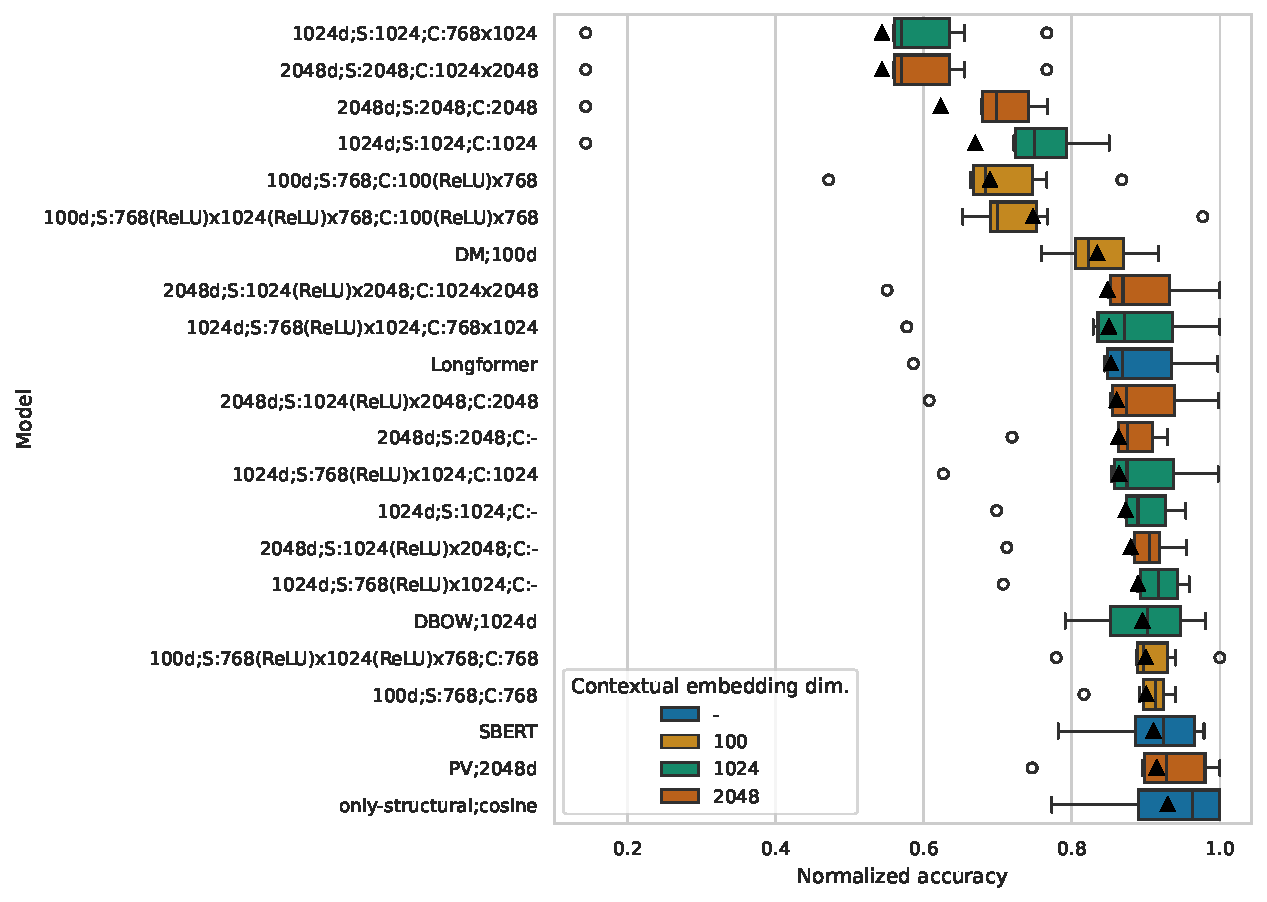
\includegraphics[width=\textwidth]{img/projections_contextual.pdf}

  \caption{Performances of student models trained with different projections
  and without structural loss. We compare the students to all the relevant
  teachers, Longformer, and \Model{only-structural;cosine}.}

  \label{fig:projections_contextual}

\end{figure}

\subsubsection{Contextual projection with cosine structural
loss}\label{section:projections_cos}

In this section, we search for the best-performing projections while
simultaneously using cosine structural loss. The training is a bit more complex
than in the previous section as here the student should distill two qualities,
each from a different teacher. So, even though the student and contextual
projections still behave equally, they may cause different outcomes.

We list all the tested projections in
Table~\ref{table:cos_contextual_projections}. We add stronger projections while
discarding some of the less successful projections from the previous section.
We again train the student models on the first 15k documents of
\Dataset{val-500k} and present the performance of the trained student models in
Figure~\ref{fig:cos_projections_contextual}. The projection variants differ
less than in the case of the student models trained without structural loss.
The cosine structural loss boosts the models' performance and lessens the
negative impact of a poor projection. As a consequence, almost all of the
student models surpass all baselines. The best-performing projections are much
larger compared to the best projections trained without any structural loss.
As the added structural loss puts more pressure on the
student, the contextual loss needs to give the model more freedom to avoid conflict between the losses, which would slow down the training.
With the larger projections, we were able to surpass
\Model{only-structural;cosine}. This shows that, with the right projections,
the student model benefits from both losses being used during training. Even if
the performance gain is not huge, we conclude that the contextual and
structural embeddings may complement each other in the right setting.

\begin{table}
  \centering
  \footnotesize

  \begin{subtable}{\textwidth}
    \centering
    \begin{tabular}{lr}
      \toprule
        & Contextual teacher's embedding dimension \\
        \cline{2-2} \\
        Projection & 100 \\
      \midrule
        Student & \TableProj{768(ReLU)x1024(ReLU)x768}  \\
        \multirow[t]{2}*{Contextual} & \TableProj{100(ReLU)x768}  \\
        & \TableProj{768} \\
      \bottomrule
    \end{tabular}
    \caption{100-dimensional contextual teacher}
  \end{subtable}
  \medskip

  \begin{subtable}{\textwidth}
    \centering
    \begin{tabular}{lrr}
      \toprule
        & \multicolumn{2}{c}{Contextual teacher's embedding dimension} \\
        \cline{2-3} \\
        Projection & 1024 & 2048 \\
      \midrule
        Student &  \TableProj{768(ReLU)x1024} & \TableProj{1024(ReLU)x2048} \\
        \multirow[t]{2}*{Contextual} &  \TableProj{1024} & \TableProj{2048} \\
        & - & - \\
      \midrule
        Student & \TableProj{768(ReLU)x4096(ReLU)x1024} & \TableProj{768(ReLU)x4096(ReLU)x2048} \\
        \multirow[t]{3}*{Contextual} & \TableProj{768(ReLU)x1024} & \TableProj{2048(ReLU)x2048} \\
        & \TableProj{1024} & \TableProj{2048} \\
        & - & - \\
      \bottomrule
    \end{tabular}

    \caption{1024 and 2048-dimensional contextual teachers}

  \end{subtable}

  \caption{All tested variants of projections with contextual loss and cosine
  structural loss. For a given contextual teacher, we delimit each group of
  projections by a horizontal line. We grid search all variants within each
  group. This results in 12 combinations of projections.}

  \label{table:cos_contextual_projections}
\end{table}

\begin{figure}

  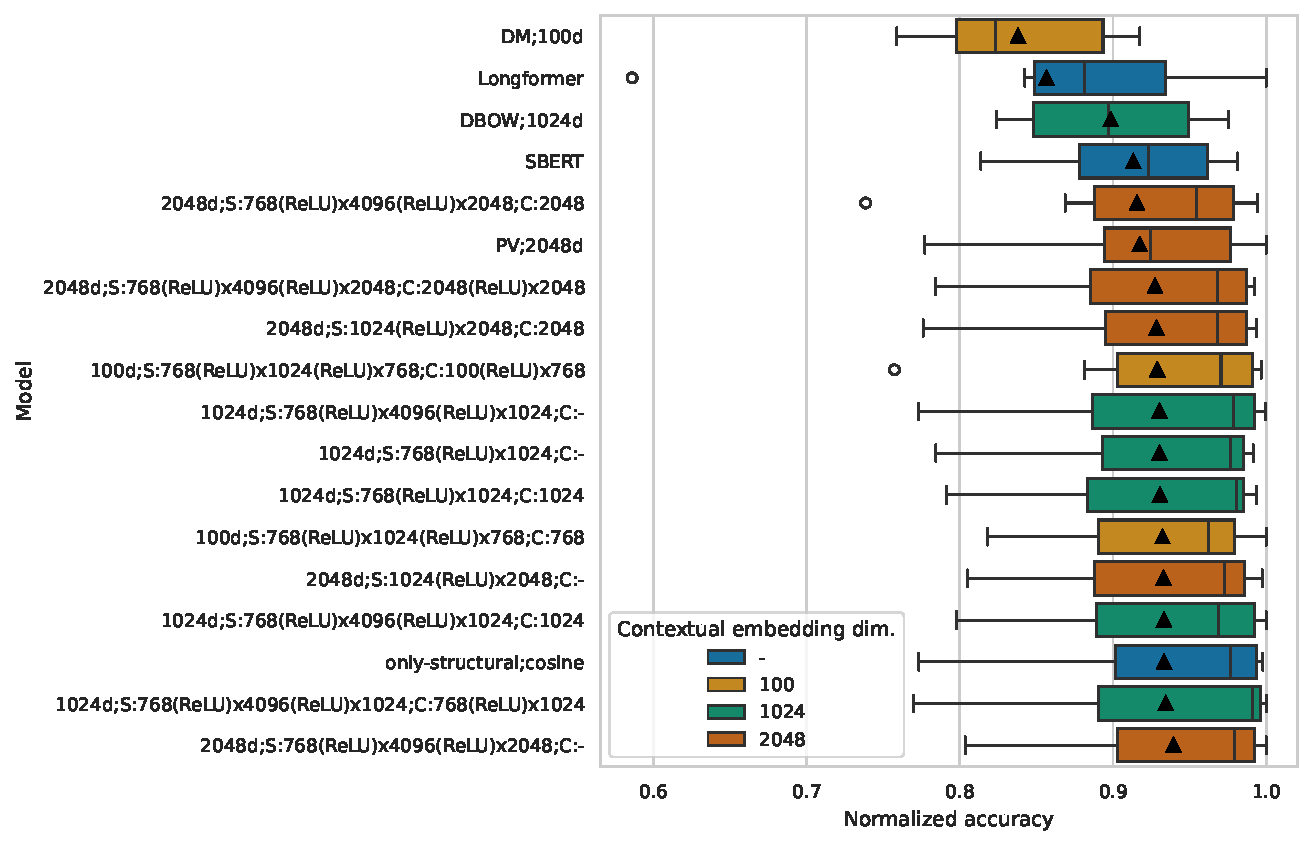
\includegraphics[width=\textwidth]{img/projections_contextual_cos.pdf}

  \caption{Performance of student models trained with contextual and cosine
  structural loss on validation tasks. We compare the student models to all
  relevant teachers, Longformer and \Model{only-structural;cosine}.}

  \label{fig:cos_projections_contextual}

\end{figure}

\subsubsection{Contextual projection with max-margin MSE structural
loss}\label{section:projections_mm_mse}

Finally, we find the optimal projections for the max-margin MSE structural
loss. We present all the tested projection variants in
Table~\ref{table:mm_mse_contextual_projections}. We include successful
projections from the previous section and add stronger contextual projections
as they perform surprisingly well in this context. Same as before, we train all
student models on the first 15k documents from \Dataset{val-500k} and compare
their performance to all relevant teachers, Longformer, and
\Model{only-structural;mm-MSE}. We present the model's performances in
Figure~\ref{fig:mm_mse_contextual_projections}. As with the cosine structural
loss, max-margin MSE loss boosts the students' performances. Consequently, the
student's performances are not as dependent on the projections as those of
students trained without structural loss. Contrary to what we witness in
previous experiments, stronger contextual projections perform very well
overall. This shows that max-margin MSE loss puts more pressure on the student's
embedding than the cosine structural loss. Despite testing even more
projections for max-margin MSE than for cosine structural loss, we fail to find
projections that would outperform \Model{only-structural;mm-MSE}. Nonetheless,
we continue experimenting with the best projections we find.

\begin{table}
  \centering
  \footnotesize

  \begin{subtable}{\textwidth}
    \centering
    \begin{tabular}{lr}
      \toprule
      % TODO: name the same in the chart or rename it here
        & Contextual teacher's embedding dimension \\
        \cline{2-2} \\
        Projection & 100 \\
      \midrule
        \multirow[t]{2}*{Student} & \TableProj{768(ReLU)x1024(ReLU)x768}  \\
        & \TableProj{768} \\
        \multirow[t]{2}*{Contextual} & \TableProj{100(ReLU)x768}  \\
        & \TableProj{768} \\
      \bottomrule
    \end{tabular}
    \caption{100-dimensional contextual teacher}
  \end{subtable}
  \medskip

  \begin{subtable}{\textwidth}
    \centering
    \begin{tabular}{lrr}
      \toprule
        & \multicolumn{2}{c}{Contextual teacher's embedding dimension} \\
        \cline{2-3} \\
        Projection & 1024 & 2048 \\
      \midrule
        Student &  \TableProj{768(ReLU)x1024} & \TableProj{1024(ReLU)x2048} \\
        \multirow[t]{3}*{Contextual} & \TableProj{768x1024} & \TableProj{1024x2048} \\
        & \TableProj{1024} & \TableProj{2048} \\
        & - & - \\
      \midrule
        Student & \TableProj{768(ReLU)x4096(ReLU)x1024} & \TableProj{768(ReLU)x4096(ReLU)x2048} \\
        \multirow[t]{3}*{Contextual} & \TableProj{1024(ReLU)x1024} & \TableProj{2048(ReLU)x2048} \\
        & \TableProj{768(ReLU)x1024} & - \\
      \bottomrule
    \end{tabular}

    \caption{1024 and 2048-dimensional contextual teachers}

  \end{subtable}

  \caption{All variants of projections tested with
  max-margin MSE structural loss. For a given contextual teacher, we delimit
  each group of projections by a horizontal line. We grid-search all variants
  within a group. This results in 14 combinations in total.}

  \label{table:mm_mse_contextual_projections}
\end{table}

\begin{figure}

  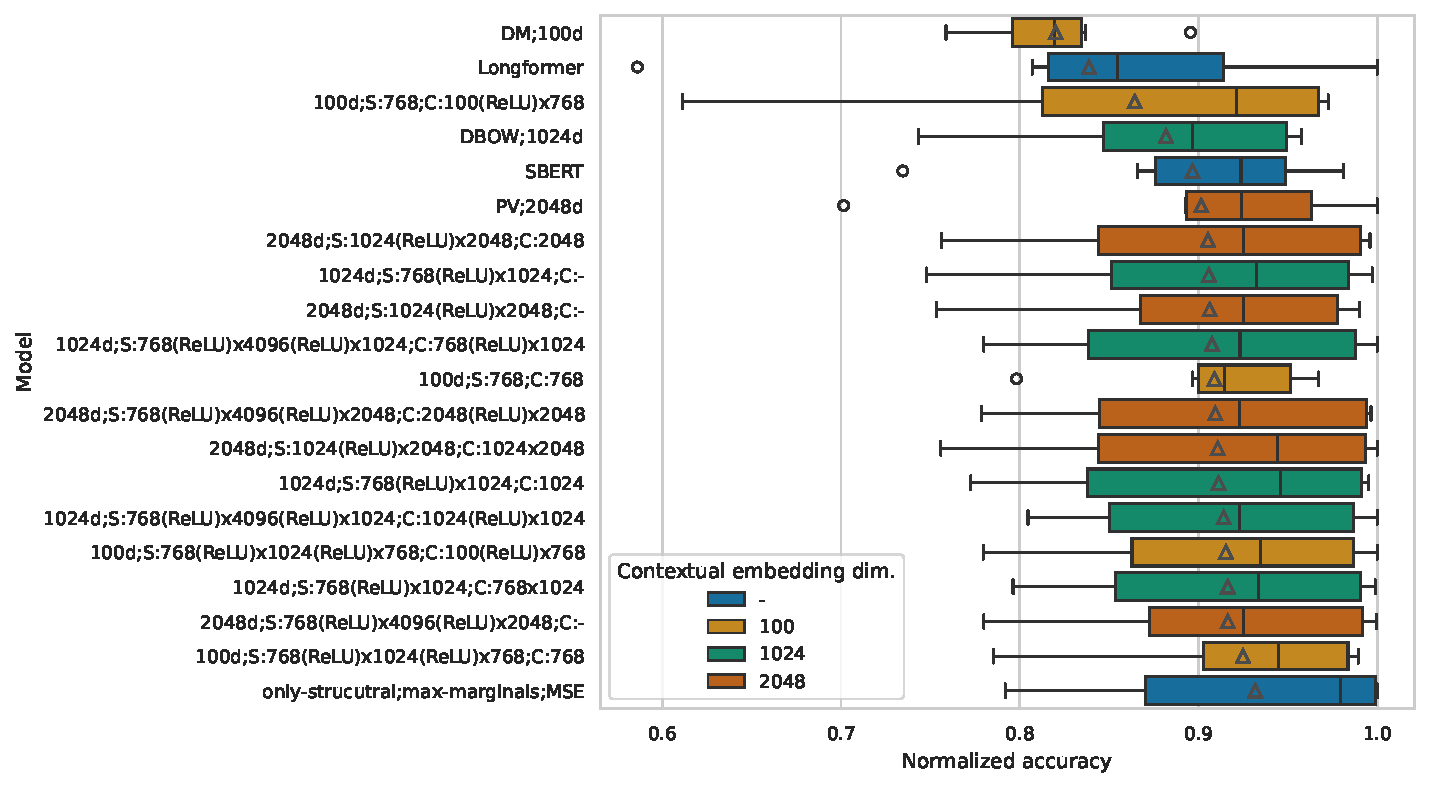
\includegraphics[width=\textwidth]{img/projections_contextual_mm_mse.pdf}

  \caption{Performance of student models trained with contextual and
  max-margin MSE structural loss on validation tasks. We compare the student
  models to all relevant teachers, Longformer and
  \Model{only-structural;mm-MSE}.}

  \label{fig:mm_mse_contextual_projections}

\end{figure}

\subsection{Weighting of structural and contextual
loss}\label{section:weighting_experiments}

The final loss is a weighted sum of the contextual and the structural loss. In
this section, we explore two weighting mechanisms. We combine a static
weighting of each loss with a dynamic masking of the structural loss based on
the length of the inputs. As the structural teacher has limited context length, its
embedding only reflects the information in the first 384 tokens. We use dynamic
masking to train the student only on those inputs, which the structural teacher
encodes whole. Therefore, in theory, the structural loss should be more
reliable. Without the masking, we might motivate the student model to focus only on the first 384 tokens and discard the rest. To summarize, we grid-search two parameters:
\texttt{max\_structural\_len} and $\lambda$. \texttt{max\_structural\_len}
determines which inputs' structural loss we mask out. $\lambda$ is the static
weight used for unmasked inputs to balance the importance of the structural and
contextual loss. For clarity, we include a Python-like pseudocode of the
weighting algorithm in Listing~\ref{lst:weighting}. Note that we mask the
inputs of the structural loss rather than its results. So, we effectively
select only some inputs on which the loss will be computed. This is especially
important for the max-margin loss, where the number of negatives effectively
decreases.

\begin{figure}
\begin{lstlisting}[caption=Python-like pseudocode of weighting algorithm.,label={lst:weighting}]
length_mask @\High{symbols}=@ torch.@\High{functions}ones@(batch_size)
if max_structural_len is not @\High{types}None\High{symbols}:@
  length_mask @\High{symbols}=@ lengths @\High{symbols}<=@ max_structural_len
lams @\High{symbols}=@ torch.@\High{functions}zeros@(batch_size).@\High{functions}fill\verb|_|@(@$\lambda$@)
lams @\High{symbols}*=@ length_mask

# For each loss we expect shape (batch_size,)
structural_loss @\High{symbols}=@ @\High{functions}\verb|structural_loss_fn|@(@\ldots@, mask=length_mask)
contextual_loss @\High{symbols}=@ @\ldots@

loss @\High{symbols}=@ structural_loss @\High{symbols}*@ lams @\High{symbols}+@ contextual_loss @\High{symbols}*@ (@\High{constants}1@ @\High{symbols}-@ lams)
loss @\High{symbols}=@ torch.@\High{functions}mean@(loss)
\end{lstlisting}
\end{figure}

In previous experiments, we weight the losses less intrusively. We do not mask
out structural loss and sum the two losses. The advantage of this approach is
that it does not reduce any gradients. However, we lose control over the mix of
the two losses. Even if the losses are not weighted, we see this as another
variant of obtaining the final loss and label it as \Model{no-weighting}. We
label all other weighting variants with the used \texttt{max\_structural\_len}
and $\lambda$ separated by a semicolon.

We consider two structural losses: cosine and max-margin MSE. For each
structural loss, we take the best-performing contextual loss from the previous
sections and try all combinations of weighting hyperparameters' values we list
in Table~\ref{table:weighting_variants}. We train a student model with each
weighting variant on the first 15k documents from \Dataset{val-500k}.

\begin{table}
  \centering
  \footnotesize
  \begin{tabular}{cc}
    \toprule
    \texttt{max\_structural\_len} & $\lambda$ \\
    \midrule
    384 & 0.95 \\
    None & 0.8 \\
    & 0.5 \\
    & 0.2 \\
    \bottomrule
  \end{tabular}

  \caption{Tested weighting hyperparameters' values. We experiment with several
  static weightings $\lambda$ with or without dynamic masking of structural
  losses for inputs longer than 385 tokens.}

  \label{table:weighting_variants}

\end{table}

\subsubsection{Weighting a contextual and the cosine structural loss}

We search for the best weighting configuration for the cosine structural loss,
\Model{PV;2048d} contextual teacher and \Proj{S:768(ReLU)x4096(ReLU)x2048;C:-}
projections, which is the most promising combination. As we mention above, we
label this combination as \Model{no-weighting}. We
present all the models' performances in Figure~\ref{fig:cos_weighting}. All the
weighting variants surpass all baselines. Interestingly, even if the weighting
is set significantly toward one side, such as \Model{None;$\lambda$=0.95} or
\Model{384;$\lambda$=0.2}, the student model can surpass the other teacher.
Therefore, the student can use the information provided by either teacher to
surpass the other one. More importantly, the best weighting variants that beat
\Model{only-structural;cosine} are more cautious with the structural loss. They
either mask it for longer documents or give it a smaller weight. Consequently,
forcing the student model to distill embedding that captures only a partial
part of its input confuses it, thereby hurting its performance.

\begin{figure}
  \centering
  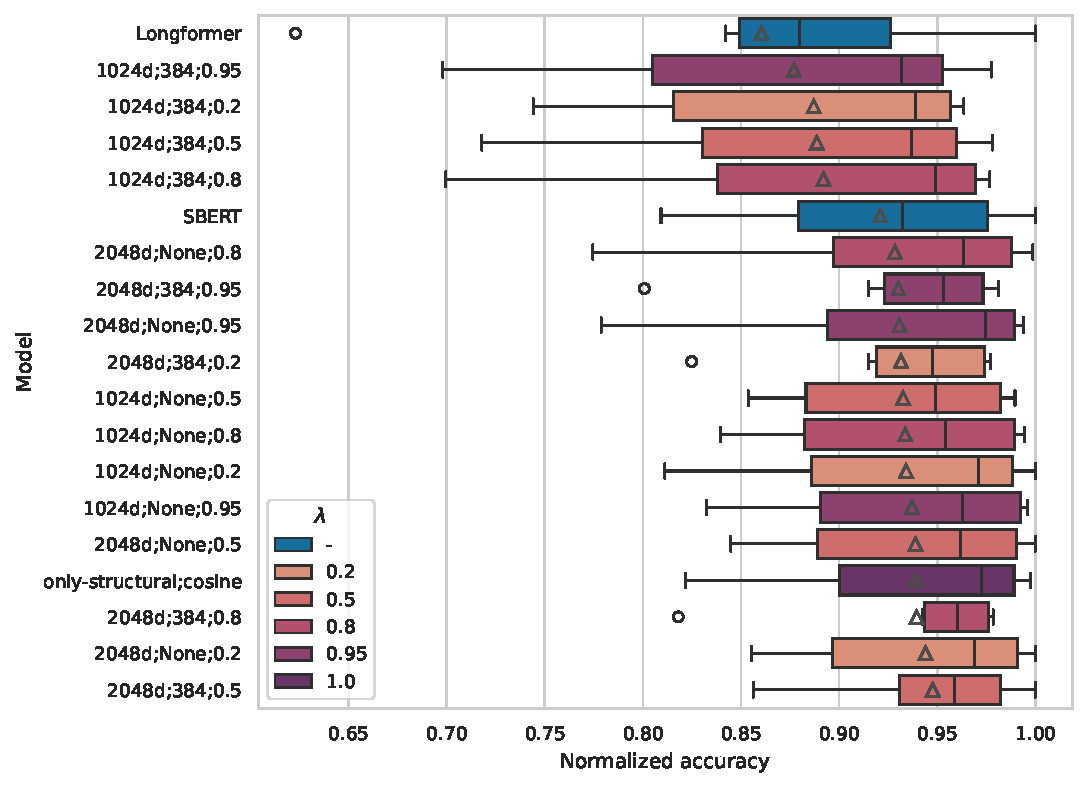
\includegraphics[width=0.85\textwidth]{img/cos_weighting.pdf}

  \caption{Performances of all weighting variants trained with cosine
  structural loss. We compare the student models to Longformer, SBERT, and
  \Model{only-structural;cosine}.}

  \label{fig:cos_weighting}

\end{figure}

We highlight the difference in performance between \Model{None;$\lambda$=0.5}
and \Model{no-weighting}. These models' losses are the same, except that
\Model{None;$\lambda$=0.5} effectively halves all loss gradients. This results
in a noticeable drop in performance. However, even with the halved gradients, \Model{384;$\lambda$=0.5} beats \Model{no-weighting} variant. This
further emphasizes the importance of masking out structural loss for long
inputs.

\subsubsection{Weighting a contextual and the max-margin MSE structural
loss}

Now we explore weighting hyperparameters for the max-margin MSE structural
loss, \Model{DM;100d} contextual teacher and
\Proj{S:768(ReLU)x1024(ReLU)x768;C:768} projections. Even though this is the best-performing combination for max-margin MSE structural loss, it does not
surpass \Model{only-structural;mm-MSE}. So, we test if different weighting of
the structural and the contextual loss can improve the score of the
\Model{no-weighting} variant. We display the models' performances in
Figure~\ref{fig:mm_mse_weighting}. Clearly, masking out some inputs' structural
loss significantly hurts performance. As we discuss in
Section~\ref{section:composite_analysis}, part of the benefit of max-margin
loss is that it increases the distance between different inputs' embeddings. If
long inputs are masked out, the loss cannot increase the margin between their
embeddings and those of the short inputs that have not been masked.
Together with the smaller number of updates, this causes the student models to
perform much worse. Note that the weighting variants with higher $\lambda$
suffer considerably more.

Even without any masking, the different loss weightings fail to improve the
score of \Model{only-structural;mm-MSE}. We highlight that
\Model{None;$\lambda$=0.5} performed a bit better than \Model{no-weighting},
which are identical, except that \Model{no-weighting} trains with
gradients twice as big. This shows that for max-margin MSE loss, the contextual teacher
does not bring any benefits. In fact, in this evaluation context, it seems that
the more we train with both losses, the worse the model will be.

\begin{figure}

  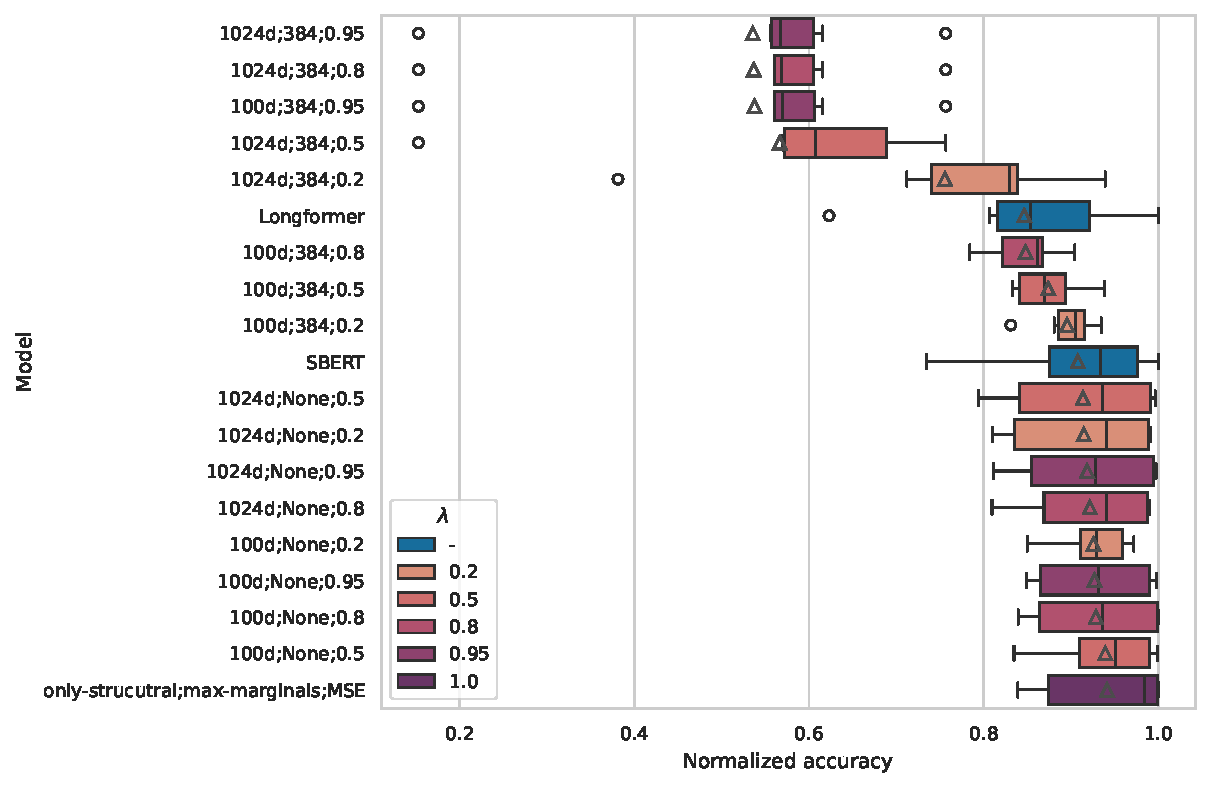
\includegraphics[width=0.9\textwidth]{img/mm_mse_weighting.pdf}

  \caption{Performances of all weighting variants for max-margin MSE
  structural loss. We compare the students to Longformer, SBERT,
  \Model{DM;100d} contextual teacher and \Model{only-structural;mm-MSE}.}

  \label{fig:mm_mse_weighting}

\end{figure}

\section{Summary}\label{section:experiments_summary}

After an extensive experimentation with our teacher-student training method, we
summarize what we test, but mainly how we interpret the results and what
conclusions we draw from them.

First, in Section~\ref{section:structural_loss}, we experiment with simple and
composite structural losses. Simple losses focus only on the similarity
between the student's and the corresponding teacher's embedding, whereas composite
losses also take advantage of the in-batch teacher's embedding of different
inputs. Cosine is the best-performing simple structural loss, surpassing even
SBERT. These results show that the combination of Longformer's architecture and
distillation of SBERT's embeddings can boost the student's performance even
above the level of the structural teacher. The best composite loss, max-margin loss with MSE used as distance, performs even better. As we show in
Section~\ref{section:composite_analysis}, with max-margin MSE loss, the student
tries to mimic the structural teacher while also increasing the distance
between its embeddings of different inputs. So, the added benefit of max-margin MSE loss compared to
cosine structural loss is a better separation between the student's embeddings.

In Section~\ref{section:structural_and_contextual}, we try to leverage the
contextual loss to improve the students even further. For our contextual loss,
we use SoftCCA loss to increase the correlation between the student's and the
contextual teacher's embeddings projected via two feed-forward networks. After
finding promising training hyperparameters for Paragraph Vector, we show that
the contextual loss alone can improve Longformer's results. Yet, it cannot
surpass SBERT or the student models trained with only the structural loss. This
demonstrates that, in our setting, the structural teacher is more important to
the student's performance than the contextual teacher. We also find the optimal
contextual loss for cosine and max-margin MSE loss. We show that the student
can benefit from both cosine structural loss and the SoftCCA contextual loss with the right projections. On the other hand, max-margin MSE loss is not as
compatible with the contextual loss. Even after many trials, we fail to find
projections that would, together with the max-margin MSE structural loss,
improve the performance of a student trained with the given structural loss
only.

We also try several ways to weigh the contextual and the structural loss. In the case of max-margin MSE structural loss, we find that even with a significant emphasis on the structural loss, the student model suffers from both the contextual loss and the max-margin MSE loss used simultaneously. Conversely, with cosine structural loss, the student model behaves intuitively. It
prefers an equal balance of the structural and the contextual loss, where the
structural loss is used only for inputs the structural teacher can encode
whole.

We demonstrate that our method can improve the student's embeddings with only about 2.5k training iterations. With the hyperparameters we listed in Table~\ref{table:student_train_params}, the student's training takes approximately 3-5 hours on a consumer-grade GPU card and requires only about 12GB of VRAM. As we see in Figure~\ref{fig:experiments_final_comparison}, with such low resource consumption, our method is able to significantly improve Longformer's performance, while also outperforming both teachers on validation tasks. For clarity, we also include the configuration of all 4 variants in
Table~\ref{table:experiments_final_config}.

\begin{figure}
    \centering
    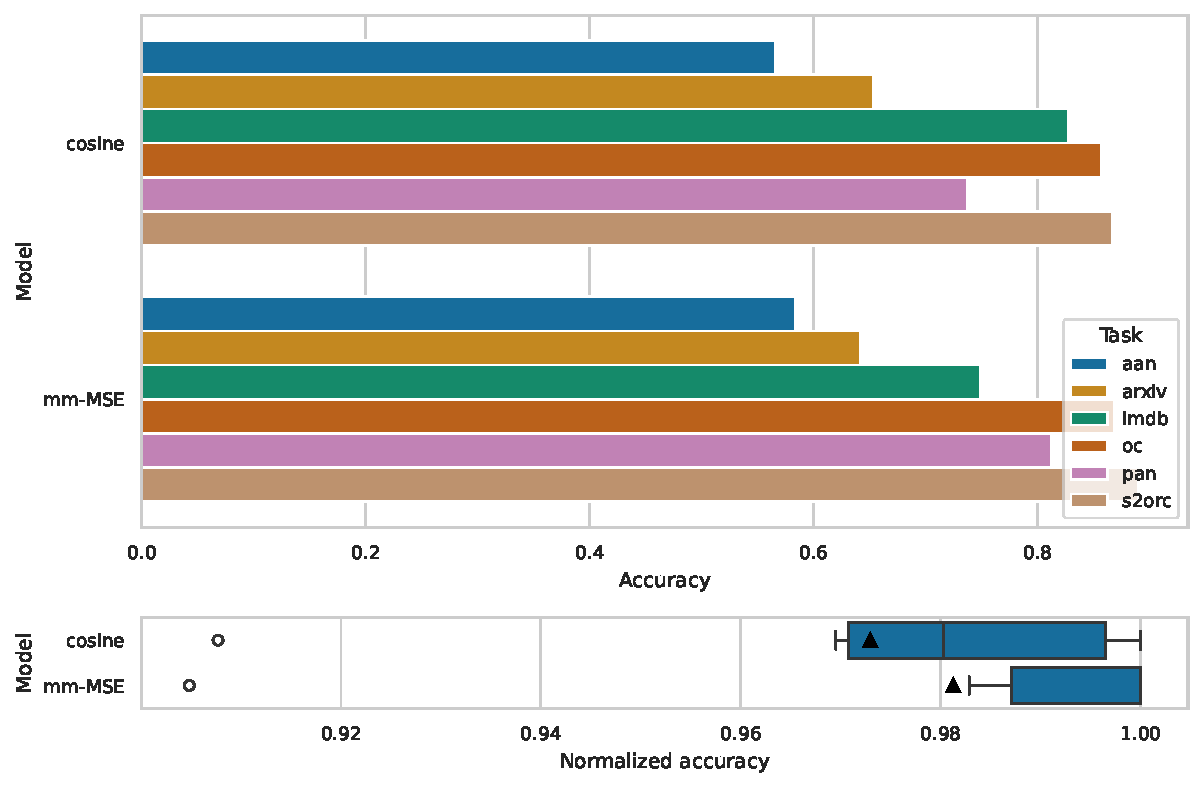
\includegraphics[width=\textwidth]{img/experiments_final_models.pdf}

    \caption{Performance of the two best student models on validation tasks per
    each structural loss. We compare the student's performances to Longformer
    and the relevant teacher models. The configuration of the student models is
    summarized in Table~\ref{table:experiments_final_config}.}

    \label{fig:experiments_final_comparison}

\end{figure}

\begin{table}

  \footnotesize
  \centering

  \begin{subtable}{\textwidth}
    \centering

    \begin{tabular}{lcc}
      \toprule
      & \multicolumn{2}{c}{Models} \\
      \cline{2-3} \\
      Hyperparameter & \TableModel{masked-cosine;$\lambda$=0.5} & \TableModel{cosine;no-weighting} \\
      \midrule
      Structural loss & \multicolumn{2}{c}{cosine distance} \\
      Contextual teacher & \multicolumn{2}{c}{\TableModel{PV;2048d}} \\
      Student projection & \multicolumn{2}{c}{\TableProj{768(ReLU)x4096(ReLU)x2048}} \\
      Contextual projection & \multicolumn{2}{c}{\TableProj{-}} \\
      Weighting $\lambda$ & 0.5 & - \\
      Structural loss masking & longer than 386 tokens & - \\
      \bottomrule
    \end{tabular}

    \caption{Models using cosine structural loss.}

  \end{subtable}
  \bigskip

  \begin{subtable}{\textwidth}
    \centering

    \begin{tabular}{lcc}
      \toprule
      & \multicolumn{2}{c}{Models} \\
      \cline{2-3} \\
      Hyperparameter & \TableModel{mm-MSE;$\lambda$=0.5} & \TableModel{only-structural;mm-MSE} \\
      \midrule
      Structural loss & \multicolumn{2}{c}{max-margin MSE} \\
      Max-margin $\gamma$ & \multicolumn{2}{c}{1} \\
      Contextual teacher & \TableModel{DM;100d} & - \\
      Student projection & \TableProj{768(ReLU)x1024(ReLU)x768} & - \\
      Contextual projection & \TableProj{768} & - \\
      Weighting $\lambda$ & 0.5 & - \\
      Structural loss masking & - & - \\
      \bottomrule
    \end{tabular}

    \caption{Models using max-margin MSE structural loss.}

  \end{subtable}

  \caption{Configurations of the best two models for each structural loss.}

  \label{table:experiments_final_config}

\end{table}
